\documentclass[12pt,onecolumn,final]{IEEEtran}

\usepackage[T1]{fontenc}
\usepackage[utf8]{inputenc}
\usepackage[brazil]{babel}
\usepackage{graphicx}
\usepackage{float}
\usepackage{geometry}
\usepackage[hidelinks]{hyperref}

\geometry{margin=2.5cm}
\graphicspath{{images/}}

\newcommand{\triplaimagem}[4]{%
    \noindent
    \begin{minipage}[t]{0.31\textwidth}
        \centering
        \includegraphics[width=\linewidth,height=3.0cm,keepaspectratio]{#1}\\
        \small Original
    \end{minipage}
    \hfill
    \begin{minipage}[t]{0.31\textwidth}
        \centering
        \includegraphics[width=\linewidth,height=3.0cm,keepaspectratio]{#2}\\
        \small Níveis de cinza
    \end{minipage}
    \hfill
    \begin{minipage}[t]{0.31\textwidth}
        \centering
        \includegraphics[width=\linewidth,height=3.0cm,keepaspectratio]{#3}\\
        \small Segmentada
    \end{minipage}
    \par\smallskip
    \centering\small\textbf{#4}\par\medskip
}

\title{Segmentação de Imagens Urbanas por Textura com Banco de Filtros Multiescala\\
\large CI1026 - Visão Computacional e Percepção}

\author{
\IEEEauthorblockN{Marcelo Gyovani Pereira (GRR20221225)\\Vinicius Evair da Silva (GRR20221251)}\\
\IEEEauthorblockA{
Graduandos do Curso de Bacharelado em Ciência da Computação\\
\textit{Departamento de Informática}\\
\textit{Universidade Federal do Paraná -- UFPR}\\
Curitiba, Brasil}
}

\begin{document}
\maketitle

\begin{abstract}
Este trabalho apresenta uma abordagem clássica para segmentação de imagens baseada em textura. As imagens são convertidas para níveis de cinza e descritas localmente pela resposta média absoluta de um banco com oito filtros em três escalas. Cada janela é representada por um vetor de 24 atributos e agrupada por \textit{K-means} com distância Euclidiana. O experimento processou 162 fotografias. Os resultados mostram que o método separa regiões com texturas visualmente distintas, embora seja sensível às bordas entre materiais e à escolha do número de grupos.
\end{abstract}

\section{Introdução}

Textura descreve padrões locais de repetição, orientação e granularidade. Ela permite distinguir materiais como concreto, asfalto, vegetação e tijolo, mesmo sem identificar os objetos da imagem.

Este trabalho segmenta fotografias por textura sem usar aprendizado profundo. As respostas de filtros em diferentes orientações e escalas são resumidas em janelas locais e comparadas em um espaço multidimensional \cite{todt}. O objetivo é agrupar janelas com comportamento semelhante; portanto, os grupos representam texturas, não classes semânticas.

\section{Metodologia}

\subsection{Imagens e pré-processamento}

Foram processadas 162 fotografias próprias, todas com recortes de $512 \times 512$ pixels. As imagens RGB são convertidas para níveis de cinza com \texttt{COLOR\_BGR2GRAY}, mantendo somente a variação espacial de intensidade.

\subsection{Banco de filtros e escalas}

O banco contém oito filtros: bordas horizontal, vertical, a $45^\circ$ e a $135^\circ$; padrão circular; cantos; Gabor; e Laplaciano. Assim, as quatro orientações e o filtro circular exigidos estão incluídos.

Cada filtro é aplicado em três escalas: a imagem original, uma versão suavizada por Gaussiana $5 \times 5$ e reduzida para $256 \times 256$, e uma terceira versão obtida pela repetição do mesmo processo, com $128 \times 128$ pixels.

Como se trata de um experimento inicial e exploratório, foram priorizados filtros clássicos, de baixo custo computacional e sem ajuste por aprendizado. Os filtros de cantos, Gabor e Laplaciano complementam os detectores direcionais ao responder, respectivamente, a junções, padrões orientados e variações locais de intensidade.

\subsection{Vetores de textura e agrupamento}

A imagem é dividida em janelas não sobrepostas de $32 \times 32$ pixels. Nas escalas reduzidas, as janelas correspondentes têm $16 \times 16$ e $8 \times 8$ pixels. Para cada filtro e escala, calcula-se a média do valor absoluto da resposta na janela. Essa operação evita o cancelamento entre respostas positivas e negativas.

Cada janela produz $8 \times 3 = 24$ atributos; uma imagem gera 256 vetores. Os vetores são agrupados por \textit{K-means} com $k=4$ e distância Euclidiana. Cada rótulo é então convertido em tom de cinza e preenchido na janela correspondente. A implementação usa OpenCV \cite{opencv} e está disponível em \url{https://github.com/viniciusevair/CI1026_VSP_T1}.

\section{Resultados}

A Figura~\ref{fig:comparacao} compara visualmente a imagem original com as
versões em grayscale e segmentada. Os arquivos usados nesta comparação são
as versões renomeadas do triângulo em \texttt{report/images}.

\begin{figure}[H]
    \centering
    \begin{minipage}{0.31\textwidth}
        \centering
        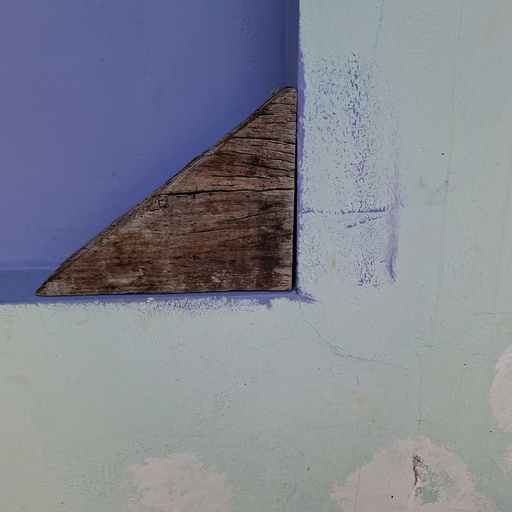
\includegraphics[width=\linewidth,height=4.5cm,keepaspectratio]{original_triangulo.jpg}

        \small Imagem original
    \end{minipage}
    \hfill
    \begin{minipage}{0.31\textwidth}
        \centering
        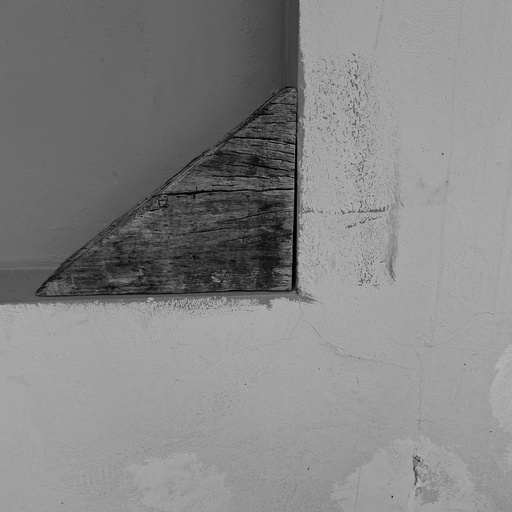
\includegraphics[width=\linewidth,height=4.5cm,keepaspectratio]{grayscale_triangulo.jpg}

        \small Imagem em grayscale
    \end{minipage}
    \hfill
    \begin{minipage}{0.31\textwidth}
        \centering
        
\includegraphics[width=\linewidth,height=4.5cm,keepaspectratio]{segmented_triangulo.jpg}

        \small Imagem segmentada
    \end{minipage}
    \caption{Comparação entre a imagem original, a conversão para grayscale e a segmentação do triângulo.}
    \label{fig:comparacao}
\end{figure}

Inclua nesta seção as observações sobre as diferenças entre as imagens e,
se aplicável, tabelas com métricas quantitativas dos resultados.

\subsection{Exemplos positivos e negativos}

Para complementar a comparação anterior, foram selecionadas imagens que
representam exemplos positivos e negativos para a análise de textura. Os
arquivos foram copiados para \texttt{report/images} com nomes descritivos.

\subsubsection{Exemplos positivos}

\begin{figure}[H]
    \centering
    \triplaimagem
        {original_arvores-ceu.jpg}
        {grayscale_arvores-ceu.jpg}
        {segmented_arvores-ceu.jpg}
        {Árvores e céu}
    \triplaimagem
        {original_muro-ceu.jpg}
        {grayscale_muro-ceu.jpg}
        {segmented_muro-ceu.jpg}
        {Muro e céu}
    \triplaimagem
        {original_muro.jpg}
        {grayscale_muro.jpg}
        {segmented_muro.jpg}
        {Muro}
    \triplaimagem
        {original_floresta.jpg}
        {grayscale_floresta.jpg}
        {segmented_floresta.jpg}
        {Floresta}
    \triplaimagem
        {original_poste-grama.jpg}
        {grayscale_poste-grama.jpg}
        {segmented_poste-grama.jpg}
        {Poste e grama}
    \caption{Exemplos positivos e suas versões em grayscale e segmentadas.}
    \label{fig:exemplos-positivos}
\end{figure}

\subsubsection{Exemplos negativos}

\begin{figure}[H]
    \centering
    \triplaimagem
        {original_meio-fio.jpg}
        {grayscale_meio-fio.jpg}
        {segmented_meio-fio.jpg}
        {Meio-fio}
    \triplaimagem
        {original_rua-grama.jpg}
        {grayscale_rua-grama.jpg}
        {segmented_rua-grama.jpg}
        {Rua e grama}
    \caption{Exemplos negativos e suas versões em grayscale e segmentadas.}
    \label{fig:exemplos-negativos}
\end{figure}

\section{Conclusão}

Apresente as principais conclusões, limitações e possíveis melhorias para o
método utilizado.


\begin{thebibliography}{9}
\bibitem{todt}
E. Todt. \textit{Computer Vision and Perception: Texture}. Departamento de Informática, Universidade Federal do Paraná, 2025.

\bibitem{humeau}
A. Humeau-Heurtier. Texture Feature Extraction Methods: A Survey. \textit{IEEE Access}, 7:8975--9000, 2019. doi: \url{https://doi.org/10.1109/ACCESS.2018.2890743}.

\bibitem{opencv}
G. Bradski. The OpenCV Library. \textit{Dr. Dobb's Journal of Software Tools}, 2000.
\end{thebibliography}
\end{document}
